% 第三章 霍普夫子 稳定性研究
\chapter{霍普夫子 稳定性研究}

阻挫交换铁磁体系中 霍普夫子 的存活情况是本章的核心议题。通过微磁学仿真,本文对该体系内 霍普夫子 维持稳态所需的前提条件、平衡尺寸的材料参数的可行区间进行了系统研究。

\section{弛豫特性与位置稳定性}

\subsection{模型设置}
本文选取的阻挫交换铁磁体系源于已有理论工作\cite{sallermann2023stability}，随后的研究在同一类体系中对 霍普夫子 的有限寿命、坍塌情况及逃逸原理开展了深入分析\cite{lobanov2023lifetime}。仿真采用的材料与几何参数汇总于\cref{tab:frustrated-params}。

\begin{table}[htbp]
  \centering
  \caption{阻挫交换铁磁体系参数。}
  \label{tab:frustrated-params}
  \begin{tabular}{lll}
    \toprule
    参数 & 符号 & 数值 \\
    \midrule
    饱和磁化强度 & $M_s$ & $\SI{1.5e5}{A/m}$ \\
    最近邻交换刚度 & $A_{\text{ex}}$ ($J_1$) & $\SI{5e-12}{J/m}$ \\
    次近邻交换 & $J_2$ & $-0.164 \, J_1$ \\
    第四近邻交换 & $J_4$ & $-0.082 \, J_1$ \\
    模型尺寸 & — & $\SI{50}{nm} \times \SI{50}{nm} \times \SI{50}{nm}$ \\
    网格 & — & $100 \times 100 \times 100$ \\
    格点间距 & — & $\SI{0.5}{nm}$ \\
    边界条件 & — & 三维周期性边界 \\
    \bottomrule
  \end{tabular}
\end{table}

本研究中霍普夫子的结构稳定性来源于阻挫交换相互作用，在仿真模型中未引入 DMI、磁晶各向异性及退磁场等额外能量项。计算域采用三维周期性边界条件（PBC），以等效表征无限体块磁性材料的物理环境。

\subsection{漂移稳定性分析}
初始构型在能量弛豫过程中的空间位置漂移特性是评估其器件应用可行性的关键因素。为此研究设计了四组控制变量对照实验（$\alpha = 0.2$、$K_{u1} = 0$、初始尺寸 $R = \SI{3}{nm}$, $r = \SI{2}{nm}$、演化时长 \SI{2}{ns} 均保持统一）,系统遍历了背景磁化方向（$m_z$、$m_x$、$m_y$）与 霍普夫子 环面轴向（$z$、$x$、$y$）的多种组合。

\cref{tab:drift-results}汇总了漂移实验的定量数据。四组配置呈现高度一致的动力学特征，霍普夫子 质心均在前 $\sim\SI{1}{ns}$ 内沿环面轴向完成约 $\SI{4.75}{nm}$ 的一次性位移,随后被格点势能锁定；与此同时,垂直于轴向的各分量在全时程内严格保持为零。该结果表明,背景磁化取向不构成影响 霍普夫子 漂移行为的因素。

\begin{table}[htbp]
  \centering
  \caption{控制变量漂移实验结果汇总（统一参数，$\alpha = 0.2$, $K_{u1} = 0$, $R_0 = \SI{3}{nm}$, $r_0 = \SI{2}{nm}$）。}
  \label{tab:drift-results}
  \begin{tabular}{ccccc}
    \toprule
    配置 & 背景方向 & 霍普夫子 轴向 & 轴向位移 & 横向位移 \\
    \midrule
    bg=$m_z$, axis=$z$ & $m_z = +1$ & $z$ & $+\SI{4.75}{nm}$ ($z$) & $\SI{0}{nm}$ \\
    bg=$m_z$, axis=$x$ & $m_z = +1$ & $x$ & $+\SI{4.75}{nm}$ ($x$) & $\SI{0}{nm}$ \\
    bg=$m_y$, axis=$y$ & $m_y = +1$ & $y$ & $+\SI{4.75}{nm}$ ($y$) & $\SI{0}{nm}$ \\
    bg=$m_x$, axis=$x$ & $m_x = +1$ & $x$ & $+\SI{4.75}{nm}$ ($x$) & $\SI{0}{nm}$ \\
    \bottomrule
  \end{tabular}
\end{table}

上述漂移现象源于连续解析模型与离散数值网格之间的失配。由解析公式生成的初始构型其几何质心通常偏离离散网格的局域能量极小点。在弛豫降能机制驱动下，霍普夫子质心向最近的能量势谷发生微小位移，该过程在初始的 \SI{1}{ns} 内达到平衡状态。位移表现出强烈的方向性，沿环面轴向的网格能量势垒较低，因而允许微小的纵向滑动。相较之下环面平面内的横向势垒较高，弛豫过程中释放的能量不足以克服该势垒，导致横向位移分量恒为零。

四组实验的总漂移距离演化曲线在误差范围内彼此重叠,与上述分析一致。为进一步研究长时行为,本文以 $m_x = +1$ 背景执行了 \SI{10}{ns} 的延长验证（\cref{fig:drift-10ns}）。结果显示,初始弛豫结束后的 \SI{9}{ns} 区间内 霍普夫子 质心未发生任何可检出的位移,$y$ 与 $z$ 两方向全程保持零漂移,由此确认了该体系的长时位置稳定性。

\begin{figure}[H]
  \centering
  
\includegraphics[width=0.75\textwidth]{figures/fig3-4_drift_trajectory_10ns.png}
  \caption{$m_x = +1$ 背景下 霍普夫子 的 \SI{10}{ns} 质心轨迹。(a) $\Delta x(t)$; (b) $\Delta y(t)$; (c) $\Delta z(t)$。}
  \label{fig:drift-10ns}
\end{figure}

\subsection{居中稳态验证}
前述漂移分析揭示,理想 霍普夫子 构型在弛豫后质心沿轴向偏离几何中心约 \SI{4.75}{nm}。后续自旋波仿真对初始态的对称性提出了更高要求,因此有必要将弛豫后构型重新居中,并对居中态的稳定性实施独立验证。

鉴于三维周期性边界条件（PBC）具备空间平移不变性，可通过坐标平移修正上述初始偏心现象。具体方法是将弛豫收敛后的三维磁化矩阵沿 $z$ 轴进行循环移位（采用 NumPy 的 \texttt{np.roll} 函数），使霍普夫子质心重新对齐至计算域中心 $(\SI{25}{nm}, \SI{25}{nm}, \SI{25}{nm})$。由于该操作属于整体坐标变换，磁构型的内部自旋排列与拓扑属性未受影响。

平移操作本身可能引入微扰,居中后构型的稳定性因此需要独立检验。本文选取三组具有代表性的各向异性配置（$K_{u1} = 0$、$\SI{10e3}{}$、$\SI{50e3}{J/m^3}$）,在 $\alpha = 0.2$ 与 PBC 条件下各演化 \SI{1}{ns},期间持续记录 霍普夫子 质心坐标与 Hopf 指数 $Q_H$（经 mumax3 内建函数 \texttt{ext\_hopfindex\_solidanglefourier} 以 Berg-Lüscher 格点法配合涌现场的傅里叶变换计算得到，是霍普夫子拓扑构型存续的严格依据）。稳态判定标准设定为 $z$ 方向漂移量 $|\Delta z| < \SI{2}{nm}$。

验证结果列于\cref{tab:centered-stability}。三组配置均满足稳态依据,其中最大漂移出现在 $K_{u1} = 0$ 时,数值仅为 $\SI{0.70}{nm}$；$K_{u1} = \SI{10e3}{J/m^3}$ 配置下漂移进一步降至 $\SI{0.019}{nm}$。

\begin{table}[htbp]
  \centering
  \caption{居中 霍普夫子 的 \SI{1}{ns} 稳态验证结果。}
  \label{tab:centered-stability}
  \begin{tabular}{ccccc}
    \toprule
    $K_{u1}$ (J/m$^3$) & $z_0$ (nm) & $z_{\text{final}}$ (nm) & $\Delta z$ (nm) & $Q_H$ ($t_0 \to t_{\text{end}}$) \\
    \midrule
    0     & 28.44 & 29.15 & $+0.70$ & $0.999 \to 0.999$ \\
    10000 & 25.07 & 25.05 & $-0.019$ & $0.999 \to 0.999$ \\
    50000 & 25.13 & 25.19 & $+0.062$ & $0.995 \to 0.995$ \\
    \bottomrule
  \end{tabular}
\end{table}

$z$ 向漂移随时间的演化曲线见\cref{fig:centered-z-drift}。$K_{u1} = 0$ 时可观察到振幅约 $\SI{1}{nm}$ 的呼吸模式振荡,但其长时均值依然处于判定阈值以内；$K_{u1} = \SI{10e3}{}$ 与 $\SI{50e3}{J/m^3}$ 两组质心则几乎完全静止。$Q_H$ 的时间演化由\cref{fig:centered-Qh-evolution}给出，三组配置的 $Q_H$ 在全时程内均稳定维持于 1 附近（波动幅度不超过 $10^{-3}$ 量级），表明霍普夫子的拓扑构型在居中之后得到了良好的保持。

多项指标的综合评估表明,$K_{u1} = \SI{10e3}{J/m^3}$ 的居中构型在位置稳定性与结构保持两个维度上均为最优,弛豫漂移带来的不确定性至此得到有效消除。后续分析即以该居中稳态为基准,转入各向异性参数对 霍普夫子 存活情况的系统研究。

\begin{figure}[H]
  \centering
  
\includegraphics[width=0.9\textwidth]{figures/fig3-8_centered_z_drift.png}
  \caption{居中 霍普夫子 的 $z$ 方向漂移随时间演化。}
  \label{fig:centered-z-drift}
\end{figure}

\begin{figure}[H]
  \centering
  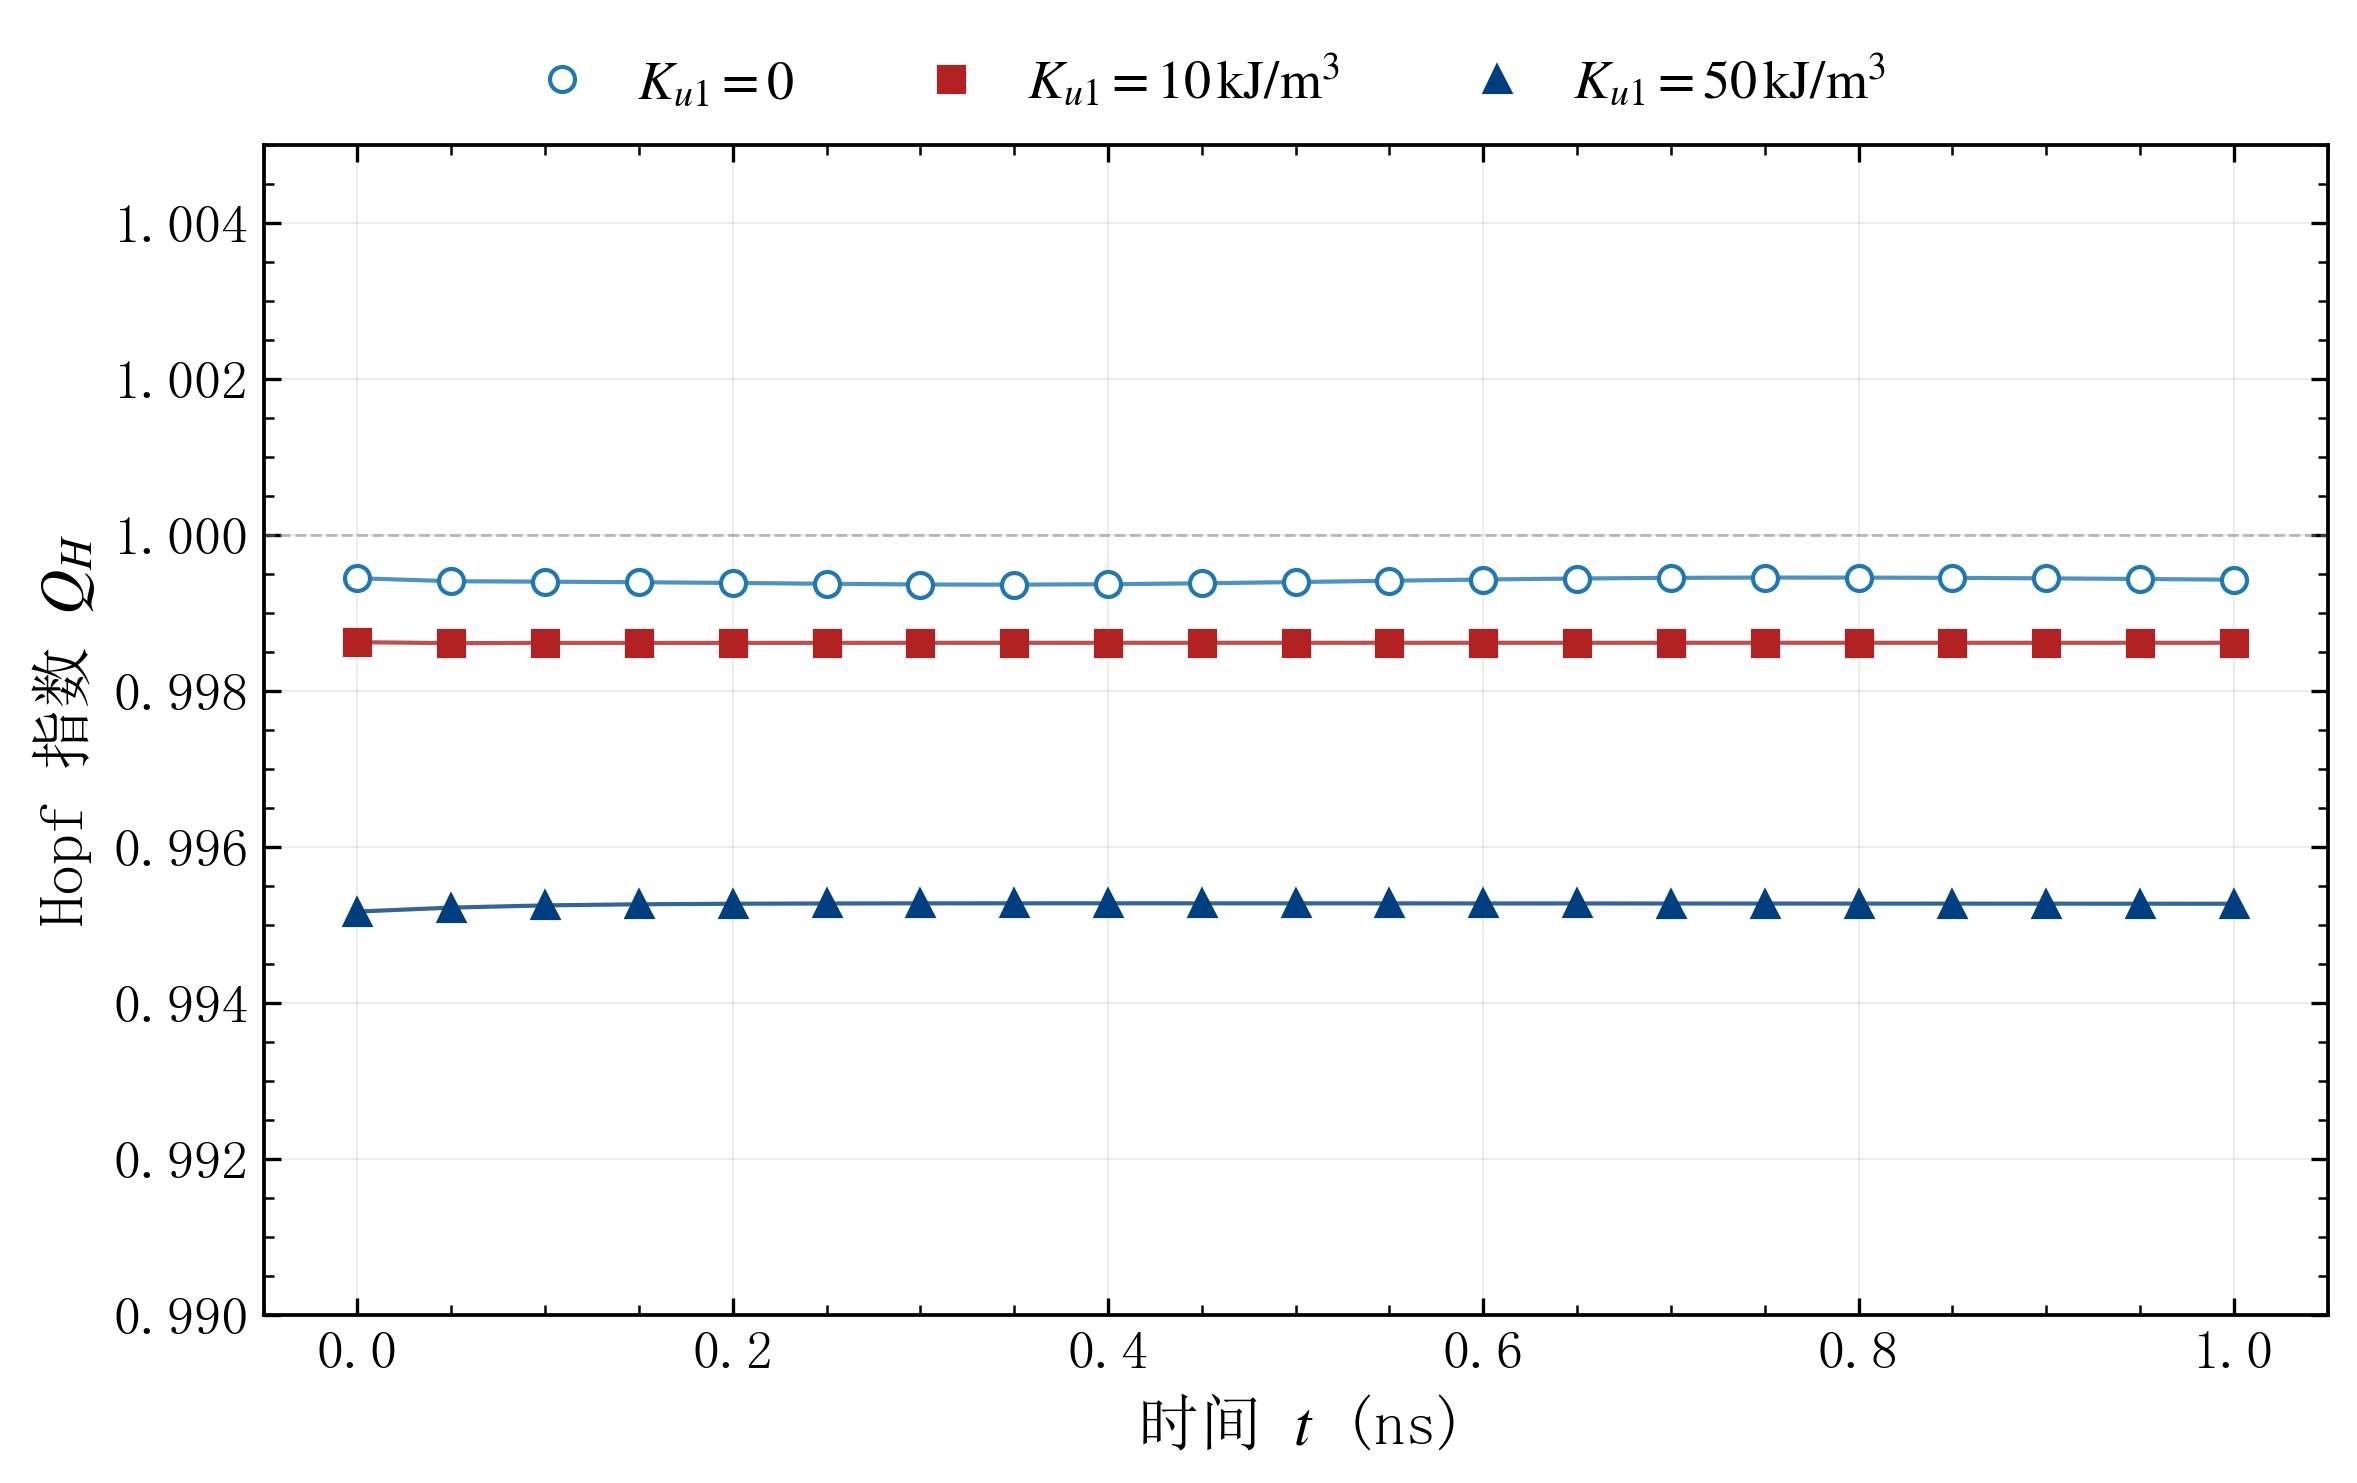
\includegraphics[width=0.9\textwidth]{figures/fig3-9_centered_Qh_evolution.png}
  \caption{居中 霍普夫子 的 Hopf 指数 $Q_H$ 随时间演化。}
  \label{fig:centered-Qh-evolution}
\end{figure}


\section{尺寸演化与临界失稳}

\subsection{各向异性对稳定性的影响}
沿 霍普夫子 环面轴向施加单轴磁晶各向异性 $K_{u1}$,其对居中稳态 霍普夫子 结构的效应是本节的研究对象。$K_{u1}$ 的扫描范围覆盖 $0 \sim \SI{75e3}{J/m^3}$,在临界区 $\SIrange{50e3}{58e3}{J/m^3}$ 处将步长加密至 $\SI{1e3}{J/m^3}$。全部实验统一以弛豫后的 $R = \SI{8}{nm}$、$r = \SI{4}{nm}$ 构型为起始条件,在 $\alpha = 0.2$ 下各演化 \SI{1}{ns}。霍普夫子存活的依据在本节采用 Hopf 指数 $Q_H$。当 $Q_H$ 维持于 $\approx 1$ 时，霍普夫子拓扑构型存续；当 $Q_H$ 塌缩为 $\approx 0$ 时，磁化场失去纽结结构并退化为均匀态。

各 $K_{u1}$ 取值下 霍普夫子 环面半径 $R$ 与管径 $r$ 的时间演化曲线由\cref{fig:anisotropy-time}给出。所有构型从同一初始尺寸出发,均在约 \SI{0.6}{ns} 内收敛至各自的平衡态。随着 $K_{u1}$ 的增大,平衡态 $R$ 与 $r$ 呈同步收缩趋势,反映出磁晶各向异性对 霍普夫子 几何结构施加的压缩效应。

$t = \SI{1}{ns}$ 时刻各组的尺寸参数与 Hopf 指数整理于\cref{tab:ku-sweep-large}。当 $K_{u1} = \SI{52e3}{J/m^3}$ 时,$Q_H$ 仍稳定于 $0.995 \approx 1$，霍普夫子拓扑构型得到维持，但管径已收缩至约 $\SI{1.2}{nm}$，仅相当于约 2.4 个格点宽度，已接近离散网格对 霍普夫子 的分辨率极限。$K_{u1}$ 升至 $\SI{55e3}{J/m^3}$ 后，$Q_H$ 塌缩至 $\approx 0$，霍普夫子 彻底失去纽结构型并退化为均匀磁化态。$K_{u1} = \SI{75e3}{J/m^3}$ 的情形更为极端，仿真在 \SI{0.37}{ns} 处即因数值发散而终止。

\begin{table}[htbp]
  \centering
  \caption{不同 $K_{u1}$ 下 霍普夫子 弛豫 \SI{1}{ns} 后的尺寸参数。}
  \label{tab:ku-sweep-large}
  \begin{tabular}{ccccc}
    \toprule
    $K_{u1}$ (J/m$^3$) & $R$ (nm) & $r$ (nm) & $Q_H$ & 状态 \\
    \midrule
    0     & 2.63 & 2.22 & 0.999 & 稳定 \\
    5000  & 2.35 & 1.85 & 0.999 & 稳定 \\
    10000 & 2.17 & 1.64 & 0.999 & 稳定 \\
    20000 & 1.82 & 1.54 & 0.998 & 稳定 \\
    30000 & 1.82 & 1.38 & 0.997 & 稳定 \\
    50000 & 1.56 & 1.24 & 0.995 & 稳定 \\
    52000 & 1.50 & 1.20 & 0.995 & 稳定（临界） \\
    55000 & —    & —    & $\approx 0$ & 坍缩 \\
    75000 & —    & —    & —     & 坍缩 \\
    \bottomrule
  \end{tabular}
\end{table}

上述结果说明该条件下的霍普夫子的临界各向异性位于 $\SI{52e3}{J/m^3}$ 与 $\SI{55e3}{J/m^3}$ 之间。

能量竞争框架为上述临界行为提供了物理解释。管径 $r$ 的平衡由三条能量通道共同决定，其中交换能 $\sim A_{\text{ex}}/r^2$ 倾向于撑大管径；阻挫交换（$J_2$、$J_4$）产生的拓扑约束将 $r$ 固定在稳态尺寸附近；各向异性能 $\sim K_{u1} r^2 L$（$L$ 为管长）则对反向磁化体积形成压缩,驱动管径收缩。

在 $K_{u1}$ 较低的区间,拓扑约束与交换能之间的对抗占据主导,$r$ 稳定在稳态尺寸附近。$K_{u1}$ 的递增使各向异性收缩项持续增强,当其数值越过 $K_{u1,c}$ 后,收缩力超过拓扑保护所能提供的抵抗,管径被压缩至格点分辨率量级（$\sim \SI{0.5}{nm}$）,离散网格无法再维持拓扑结构的完整性,霍普夫子 随即坍缩。这一结论与已有针对螺旋磁体 霍普夫子 椭圆稳定性的理论分析在定性层面相一致\cite{metlov2025elliptical}。$R$ 和 $r$ 随 $K_{u1}$ 单调递减的趋势以及临界区间的位置由\cref{fig:anisotropy-summary}直观展示。

\begin{figure}[H]
  \centering
  
\includegraphics[width=\textwidth]{figures/fig3-7_anisotropy_summary.png}
  \caption{$t = \SI{1}{ns}$ 时 霍普夫子 尺寸参数随 $K_{u1}$ 的变化。(a) 大半径 $R$; (b) 管半径 $r$。}
  \label{fig:anisotropy-summary}
\end{figure}

\clearpage

\begin{figure}[H]
  \centering
  
\includegraphics[width=\textwidth]{figures/fig3-6_anisotropy_Rr_vs_time.png}
  \caption{不同 $K_{u1}$ 下 霍普夫子 尺寸参数的时间演化。(a) 大半径 $R(t)$; (b) 管半径 $r(t)$。}
  \label{fig:anisotropy-time}
\end{figure}

\subsection{稳态尺寸}
接下来需要测试霍普夫子的稳态尺寸是否与其初态尺寸相关。测试方案为以多组不同初始尺寸（环面半径 $R$ 与管径 $r$）分别构造 霍普夫子 起始态,统一在高阻尼 $\alpha = 5.0$ 下弛豫至稳态,再由 Python 脚本提取弛豫后的几何参数。

收敛测试结果呈现于\cref{fig:size-convergence}。无论初始尺寸如何选取（$R = 3 \sim \SI{12}{nm}$, $r = 2 \sim \SI{5}{nm}$），弛豫后全部构型均收敛至同一组平衡尺寸 $R_{\text{eq}} = \SI{2.60}{nm}$ 与 $r_{\text{eq}} = \SI{2.16}{nm}$。上述结果表明，在本文所用参数条件下，体系存在唯一的稳态尺寸，霍普夫子 的平衡几何完全由材料参数决定，不受初始条件左右。这也从能量景观的角度解释了为何给定一组各向异性参数后,稳态仅对应单一特征尺寸的 霍普夫子。在多组配置的综合比较中,$K_{u1} = \SI{10e3}{J/m^3}$ 的居中构型在各项评价指标上均表现最优,本文将其选定为第五章自旋波驱动仿真的标准初始态。

\begin{figure}[H]
  \centering
  
\includegraphics[width=0.75\textwidth]{figures/fig3-3_size_convergence.png}
  \caption{尺寸收敛性测试。(a) 大半径 $R(t)$; (b) 管半径 $r(t)$。}
  \label{fig:size-convergence}
\end{figure}


本章探讨了阻挫交换铁磁体系中霍普夫子的能量弛豫特性及结构稳定边界。多组控制变量实验证实，背景磁化取向不会改变理想构型在弛豫早期的轴向微小漂移模式。采用循环移位方法实现了构型居中，并验证了具有特定磁晶各向异性（$K_{u1} = \SI{10e3}{J/m^3}$）的霍普夫子能够在长时演化中保持零漂移的优异稳定性。数值扫描确定了维持三维拓扑纽结构型的临界各向异性阈值区间为 $\num{52e3}$ 至 $\num{55e3} \, \si{J/m^3}$。此外仿真表明该物理体系下霍普夫子存在唯一的稳态尺寸，其最终几何参数仅由材料固有属性决定，与初始设定尺度无关。后续章节的自旋波驱动模拟均以本章提取的 $K_{u1} = \SI{10e3}{J/m^3}$ 居中稳定构型作为初始输入。
